\chapter{Appendices for Chapter 5}
\resumetocwriting
\section{EMScan: A Mobile Application for Assisting With Early Lyme Disease Diagnosis}\label{sec:emscan-desc}
Figure~\ref{app_workflow} shows the overall workflow of the EMScan mobile application. First, the user takes a photo of the skin lesion using the mobile camera. Second, the application automatically detects and crops the skin lesion which can be also manually adjusted by the user. Third, patient data related to the skin lesion is acquired through a series of questions and answers. Fourth, the lesion image is analyzed by a CNN image classifier, and the patient data is analyzed by the elicited statistical model to obtain two probabilities. Finally, a disease prediction with suggestion is provided to the user based on the analysis of skin lesion image and patient data. The application also provides the user with necessary details about Lyme disease and collects data with the patient’s consent for research purposes.
\begin{figure}[htb!]
	\begin{center}
		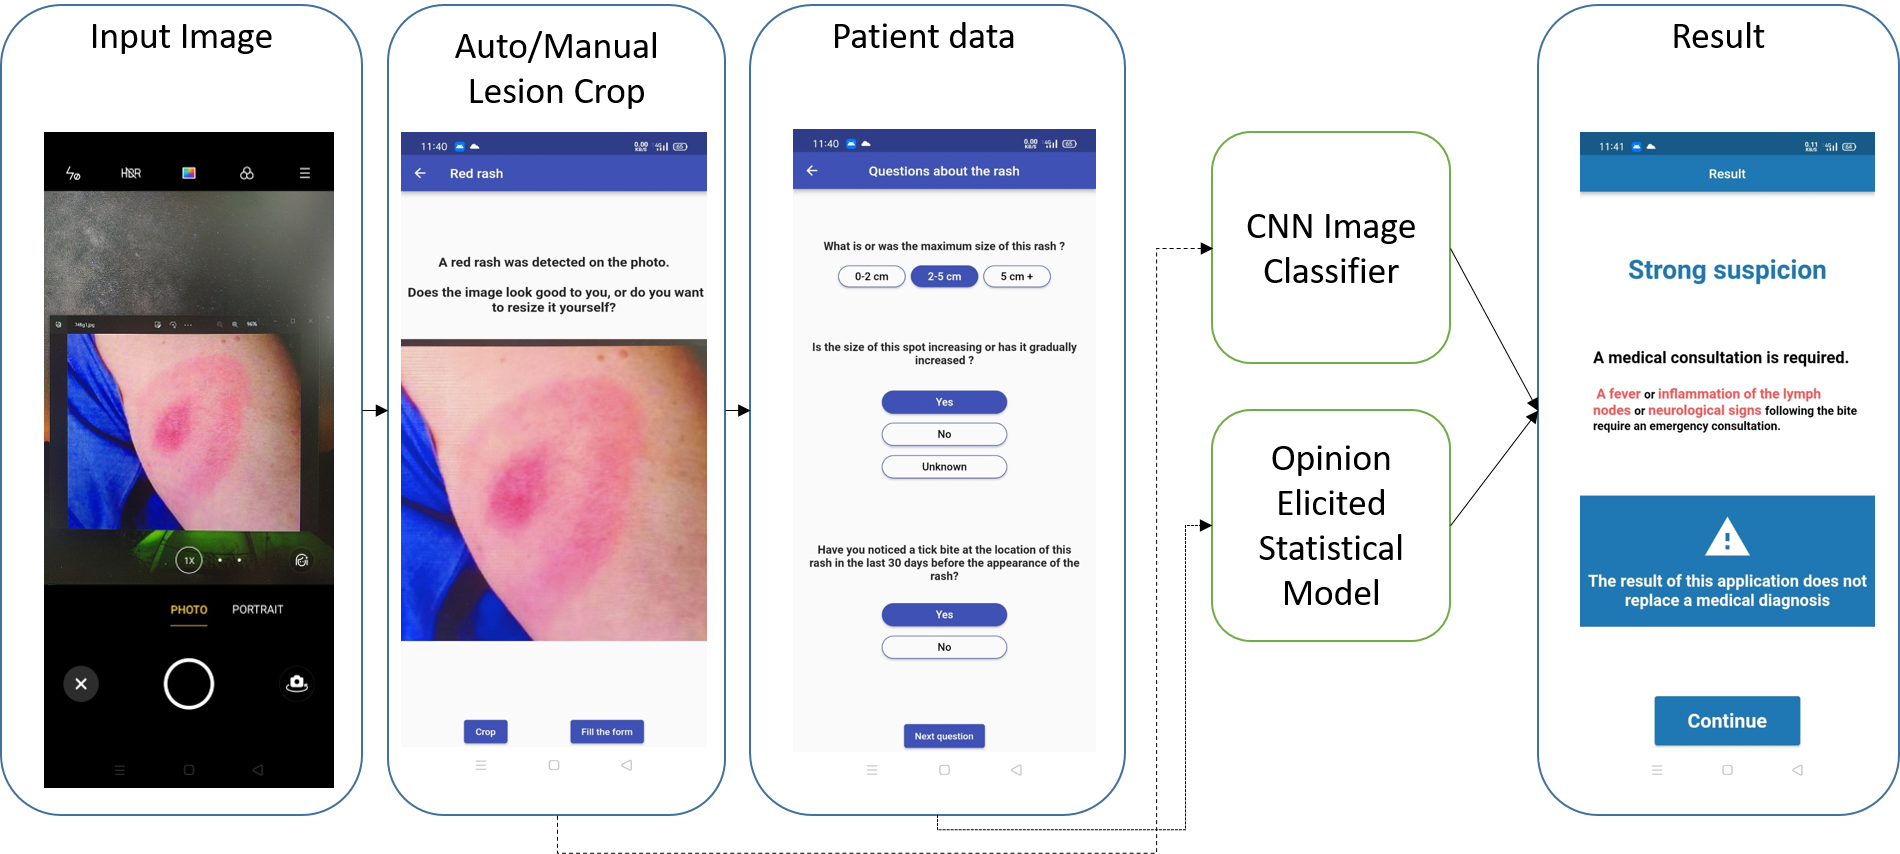
\includegraphics[width=\textwidth,keepaspectratio]{images/ongoing/app_workflow.png}
		\caption{EMScan application workflow.} \label{app_workflow}
	\end{center}
\end{figure}
\vfill\clearpage
\section{Supplementary Data for Custom Architecture}\label{sec:app-supply-custom}
This section provides detailed five-fold cross validation results of the custom architecture and the ResNet50-141 model for the updated Lyme dataset.
\stoptocwriting
\subsection{Custom Architecture}
\begin{table}[h!]
	\centering
	\caption{Five-fold cross-validation performance metrics of custom model.}
	\resizebox{\textwidth}{!}{%
		\begin{tabular}{llllllllllll}
			\toprule
			& \multicolumn{11}{c}{\textbf{Metric}}    \\ \cmidrule(l){2-12} 
			\multicolumn{1}{l}{\textbf{Fold}} & \rotatebox{45}{Accuracy} & \rotatebox{45}{Sensitivity} & \rotatebox{45}{Specificity} & \rotatebox{45}{Precision} & \rotatebox{45}{NPV} & \rotatebox{45}{MCC} & \rotatebox{45}{Kappa} & \rotatebox{45}{LR$+$} & \rotatebox{45}{LR$-$} & \rotatebox{45}{F1-Score} & \rotatebox{45}{AUC}  \\ \midrule
			fold1    & 80.57 & 82.07 & 78.92 & 81.18 & 79.88 & 0.6102 & 0.6102 & 3.8922 & 0.2273 & 0.8162 & 0.8783 \\
			fold2    & 88.29 & 89.67 & 86.75 & 88.24 & 88.34 & 0.765  & 0.7649 & 6.7663 & 0.119  & 0.8895 & 0.9447 \\
			fold3    & 86.29 & 85.87 & 86.75 & 87.78 & 84.71 & 0.7255 & 0.7253 & 6.4792 & 0.1629 & 0.8681 & 0.9221 \\
			fold4    & 84.86 & 91.85 & 77.11 & 81.64 & 89.51 & 0.7005 & 0.6943 & 4.0123 & 0.1057 & 0.8645 & 0.9151 \\
			fold5    & 83.38 & 85.79 & 80.72 & 83.07 & 83.75 & 0.6667 & 0.6663 & 4.4505 & 0.176  & 0.8441 & 0.9152 \\ \cmidrule(lr){1-12} 
			average & 84.68 & 87.05 & 82.05 & 84.38 & 85.24 & 0.6936 & 0.6922 & 5.1201 & 0.1582 & 0.8565 & 0.9151 \\
			std. deviation  & 2.62  & 3.4   & 4     & 3.03  & 3.44  & 0.0526 & 0.0525 & 1.2442 & 0.0434 & 0.0248 & 0.0214 \\
			\bottomrule
		\end{tabular}%
	}
\end{table}

\begin{figure}[h!]
	\centering
	\begin{subfigure}[b]{0.49\textwidth}
		\centering
		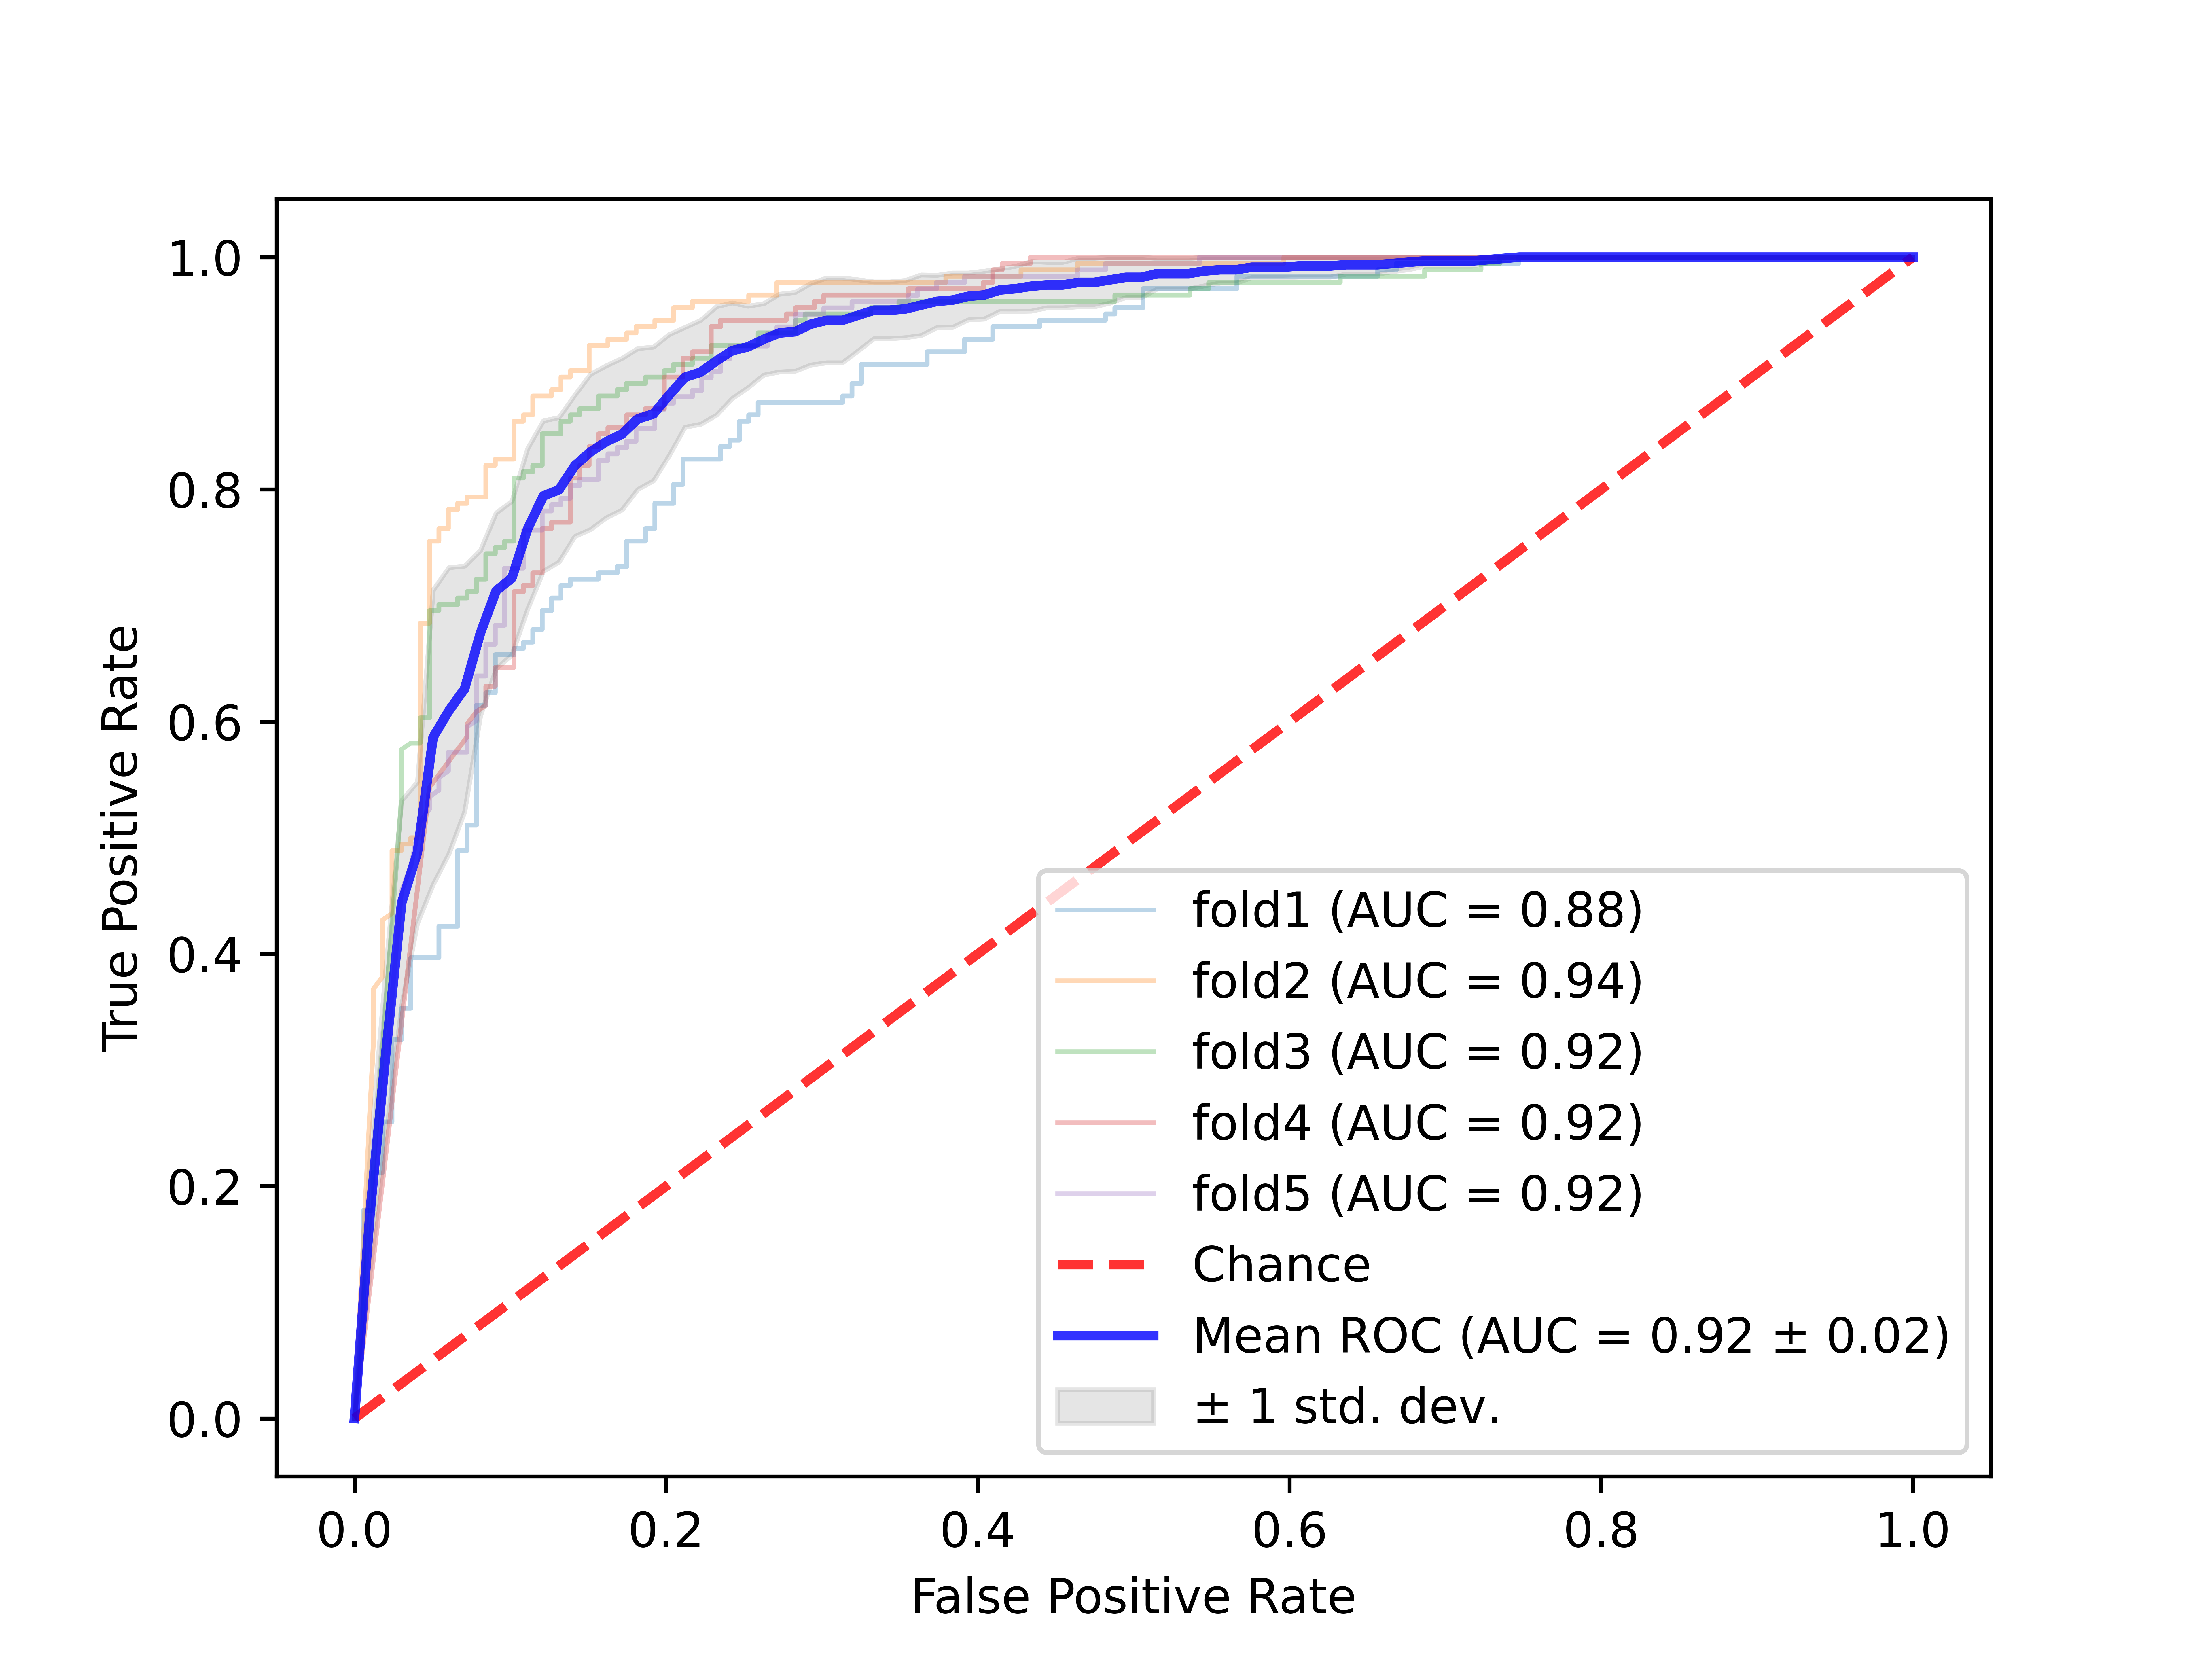
\includegraphics[width=\textwidth,keepaspectratio]{images/ongoing/custom_roc.png}
		\caption{ROC curve.}
	\end{subfigure}
	\hfill
	\begin{subfigure}[b]{0.49\textwidth}
		\centering
		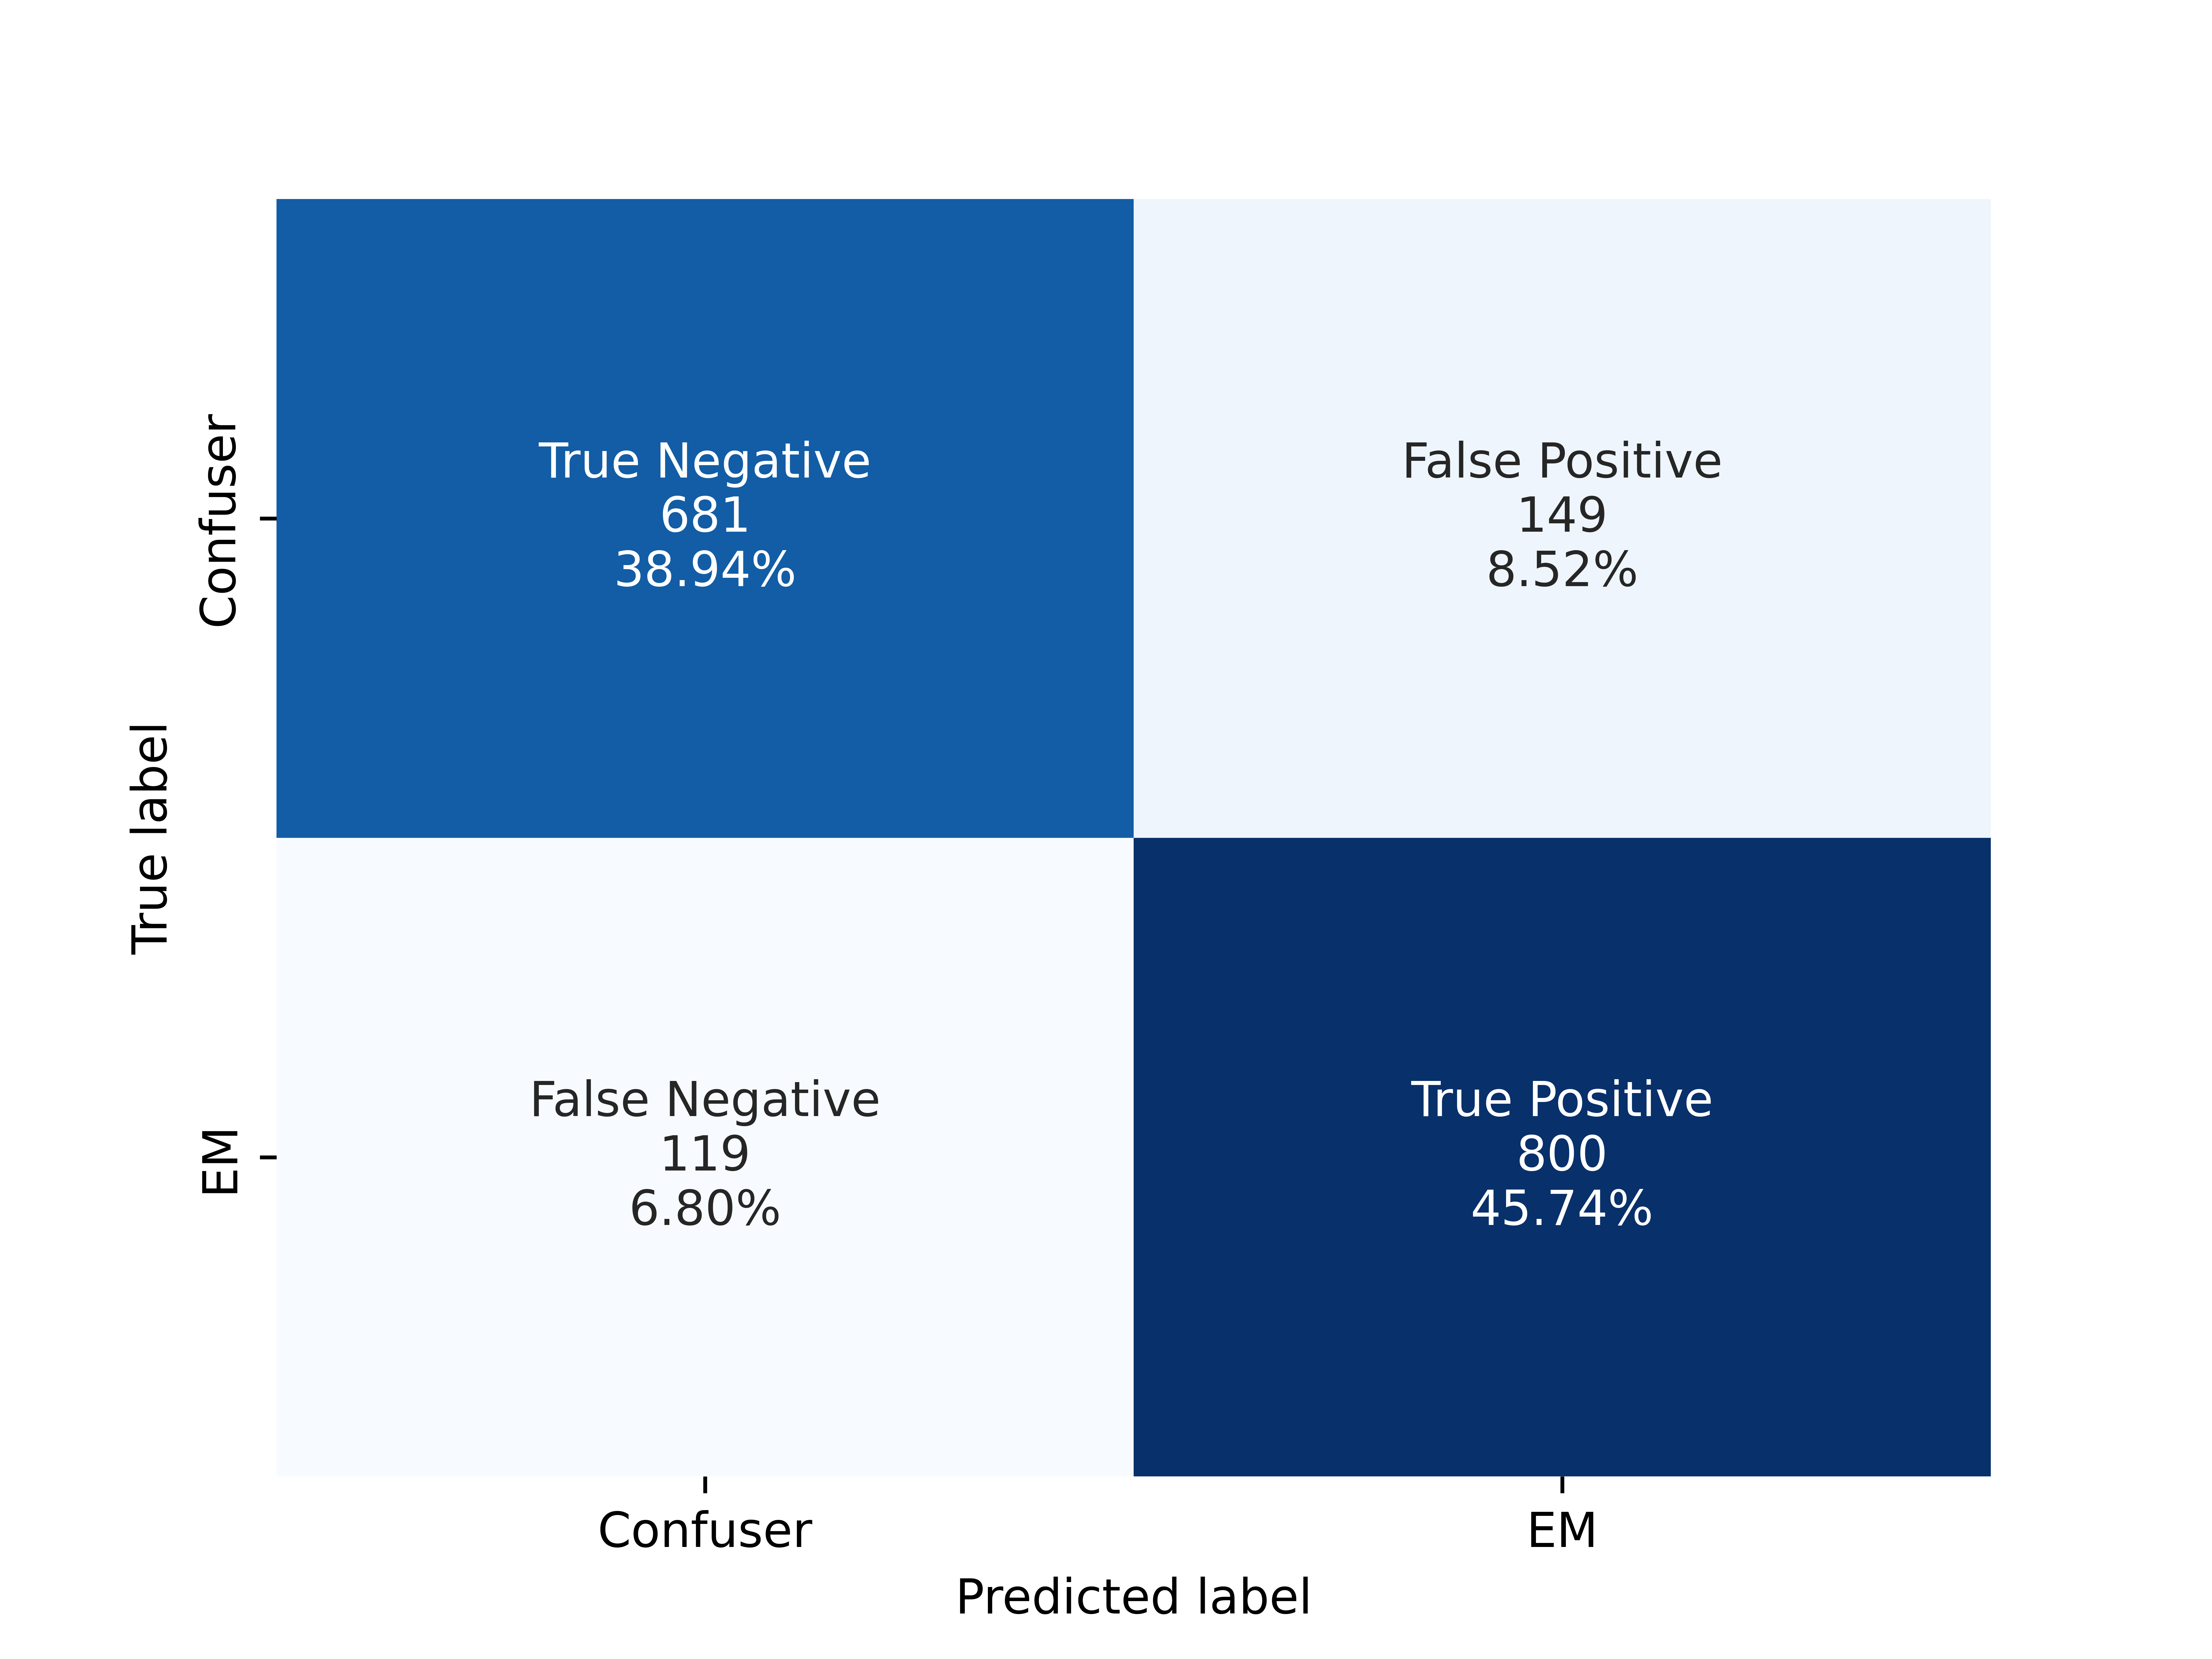
\includegraphics[width=\textwidth,keepaspectratio]{images/ongoing/custom_CM.png}
		\caption{Confusion matrix.}
	\end{subfigure}
	\caption{Five-fold cross-validation ROC curve and confusion matrix of custom model.}
\end{figure}
\vfill\clearpage
%%%%%%%%%%%%%%Break%%%%%%%%%%%%%%%%%%%%%%
%\vfill\clearpage
\subsection{ResNet50-141}
\begin{table}[h!]
	\centering
	\caption{Five-fold cross-validation performance metrics of VGG19-13 model.}
	\resizebox{\textwidth}{!}{%
		\begin{tabular}{llllllllllll}
			\toprule
			& \multicolumn{11}{c}{\textbf{Metric}}    \\ \cmidrule(lr){2-12} 
			\multicolumn{1}{l}{\textbf{Fold}} & \rotatebox{45}{Accuracy} & \rotatebox{45}{Sensitivity} & \rotatebox{45}{Specificity} & \rotatebox{45}{Precision} & \rotatebox{45}{NPV} & \rotatebox{45}{MCC} & \rotatebox{45}{Kappa} & \rotatebox{45}{LR$+$} & \rotatebox{45}{LR$-$} & \rotatebox{45}{F1-Score} & \rotatebox{45}{AUC}  \\ \midrule
			fold1    & 84.57 & 85.33 & 83.73 & 85.33 & 83.73 & 0.6906 & 0.6906 & 5.246  & 0.1752 & 0.8533 & 0.9203 \\
			fold2    & 85.43 & 88.04 & 82.53 & 84.82 & 86.16 & 0.7078 & 0.7072 & 5.0397 & 0.1449 & 0.864  & 0.9259 \\
			fold3    & 83.14 & 86.41 & 79.52 & 82.38 & 84.08 & 0.6619 & 0.6611 & 4.219  & 0.1709 & 0.8435 & 0.9148 \\
			fold4    & 84.29 & 86.96 & 81.33 & 83.77 & 84.91 & 0.6848 & 0.6842 & 4.6564 & 0.1604 & 0.8533 & 0.9194 \\
			fold5    & 86.82 & 90.71 & 82.53 & 85.13 & 88.96 & 0.7366 & 0.7349 & 5.1924 & 0.1126 & 0.8783 & 0.935  \\ \cmidrule(lr){1-12} 
			average & 84.85 & 87.49 & 81.93 & 84.29 & 85.57 & 0.6963 & 0.6956 & 4.8707 & 0.1528 & 0.8585 & 0.9231 \\
			std. deviation  & 1.23  & 1.83  & 1.42  & 1.09  & 1.89  & 0.0249 & 0.0246 & 0.3856 & 0.0227 & 0.0118 & 0.0069\\
			\bottomrule
		\end{tabular}%
	}
\end{table}

\begin{figure}[htb!]
	\centering
	\begin{subfigure}[b]{0.49\textwidth}
		\centering
		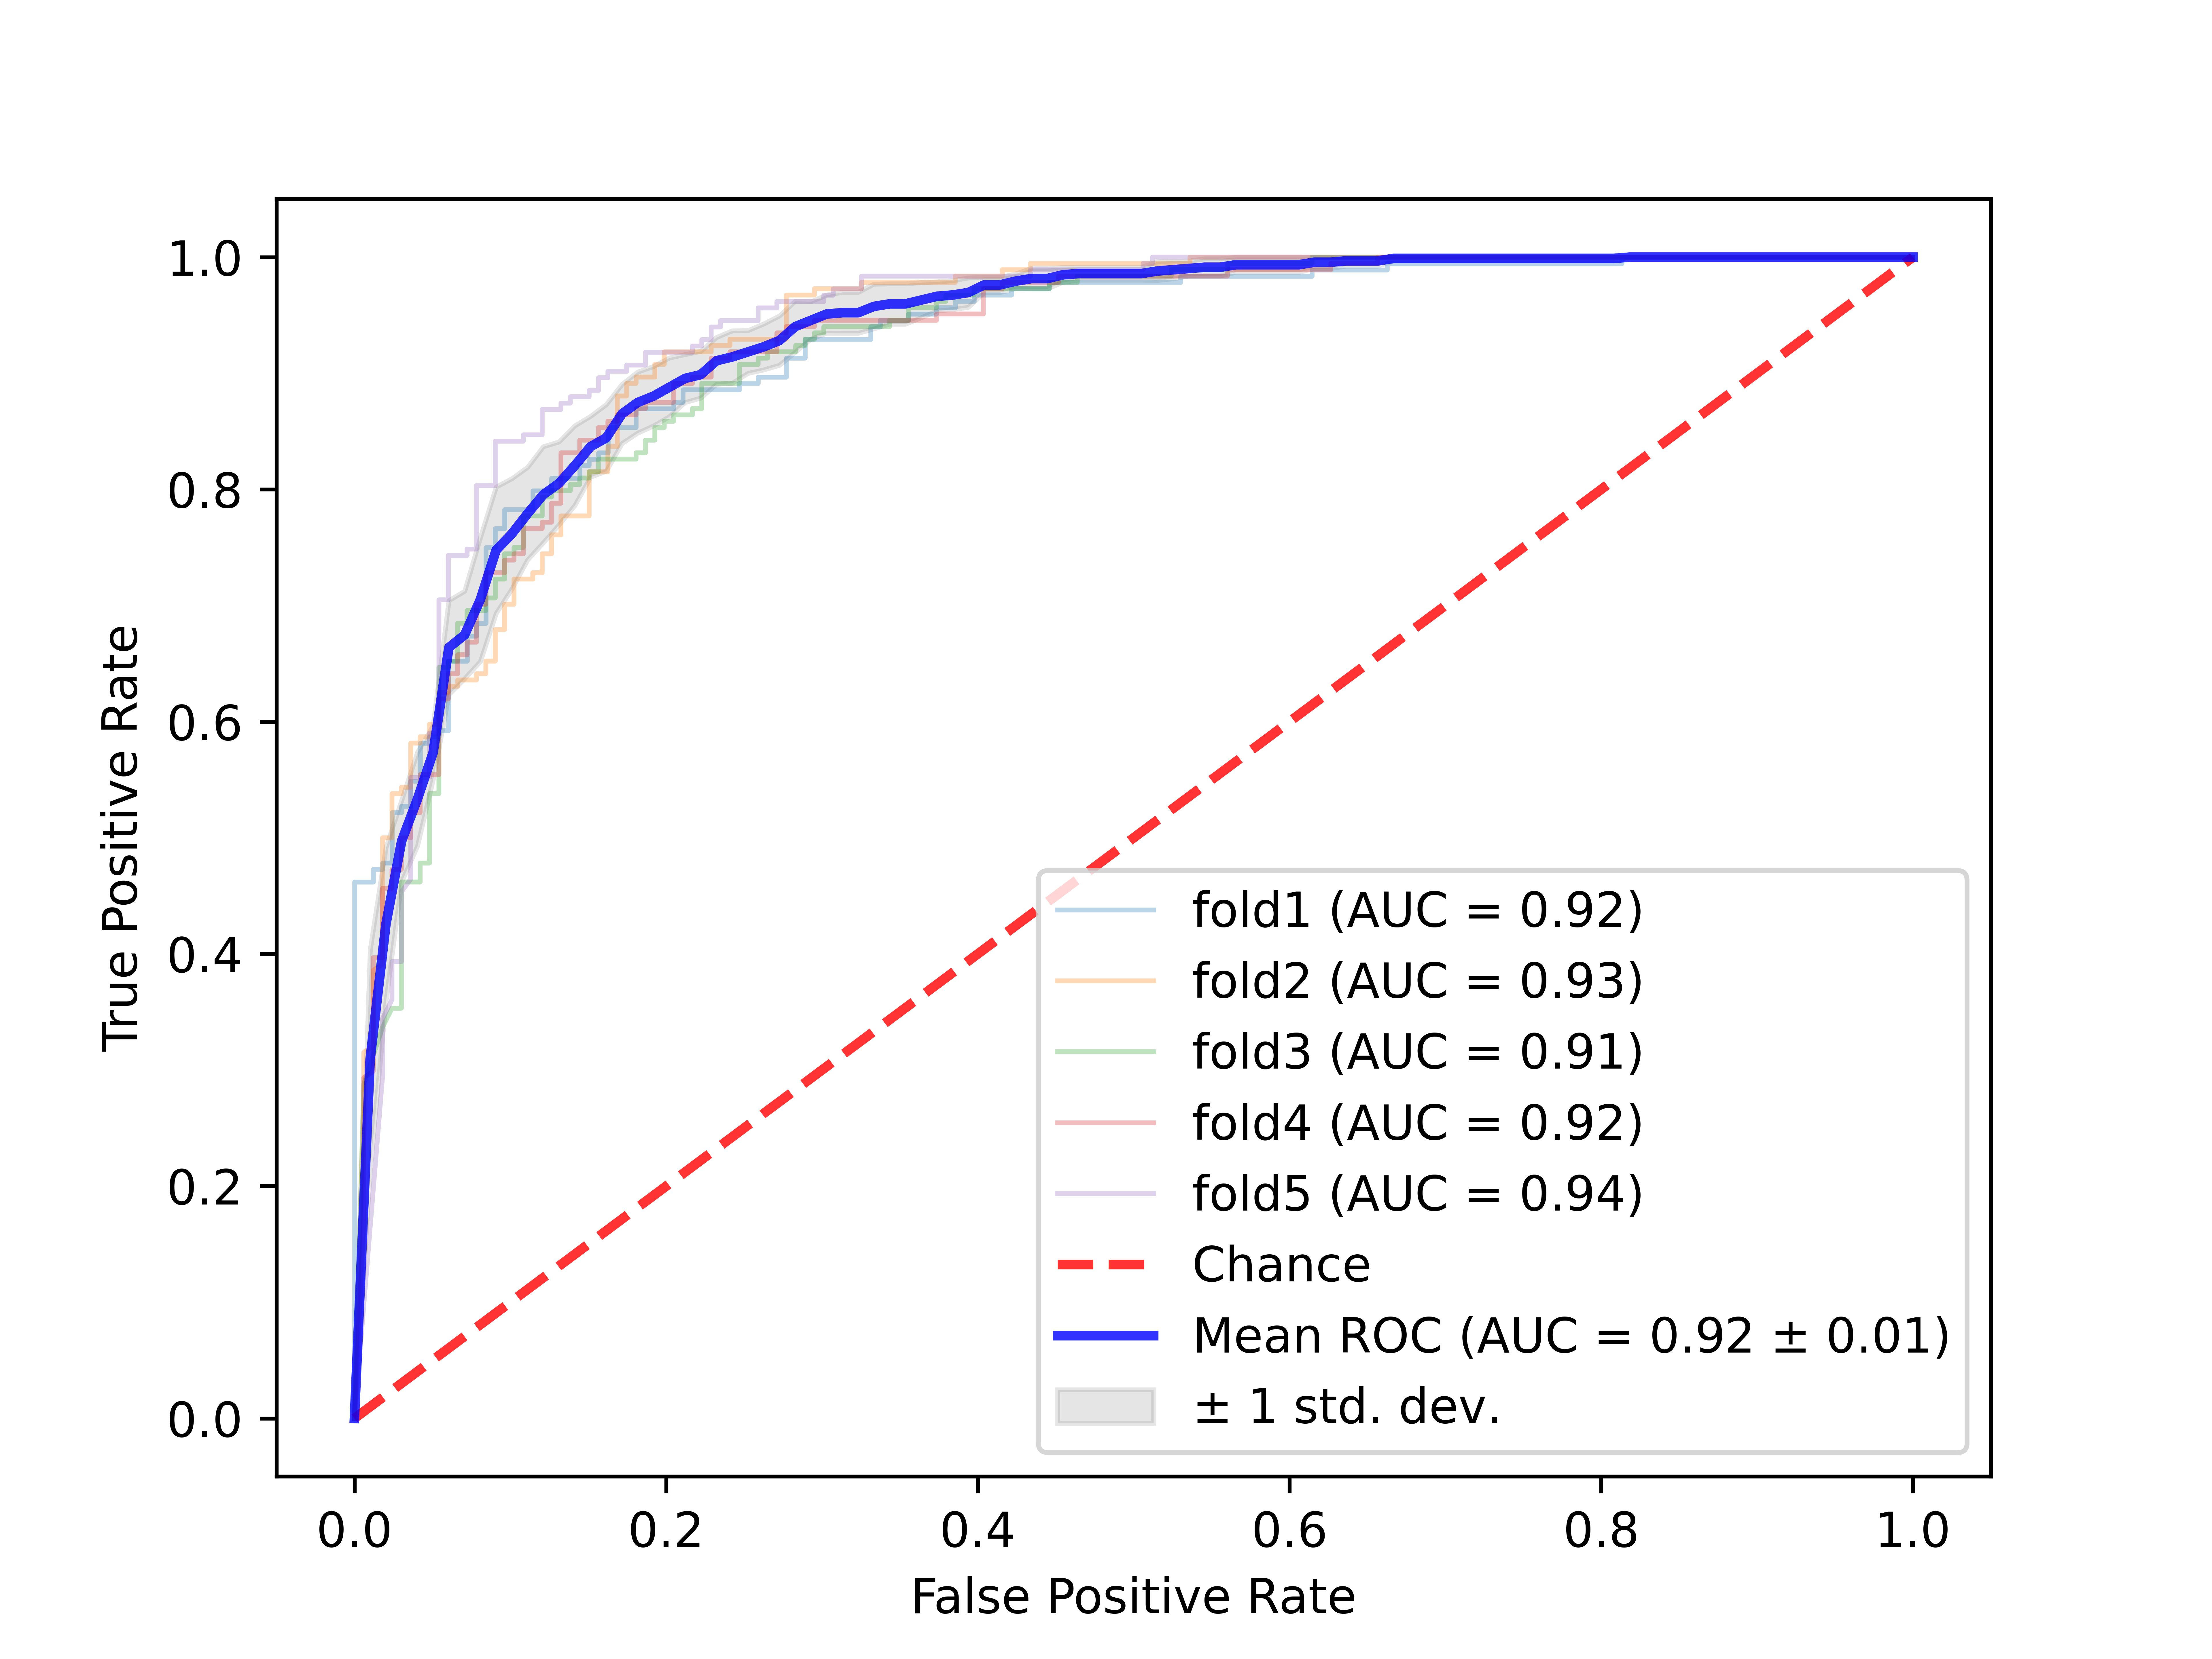
\includegraphics[width=\textwidth,keepaspectratio]{images/ongoing/ResNet50HAMIMGCOPYWEIGHTEC141DSV2logit_MultiROC.png}
		\caption{ROC curve.}
	\end{subfigure}
	\hfill
	\begin{subfigure}[b]{0.49\textwidth}
		\centering
		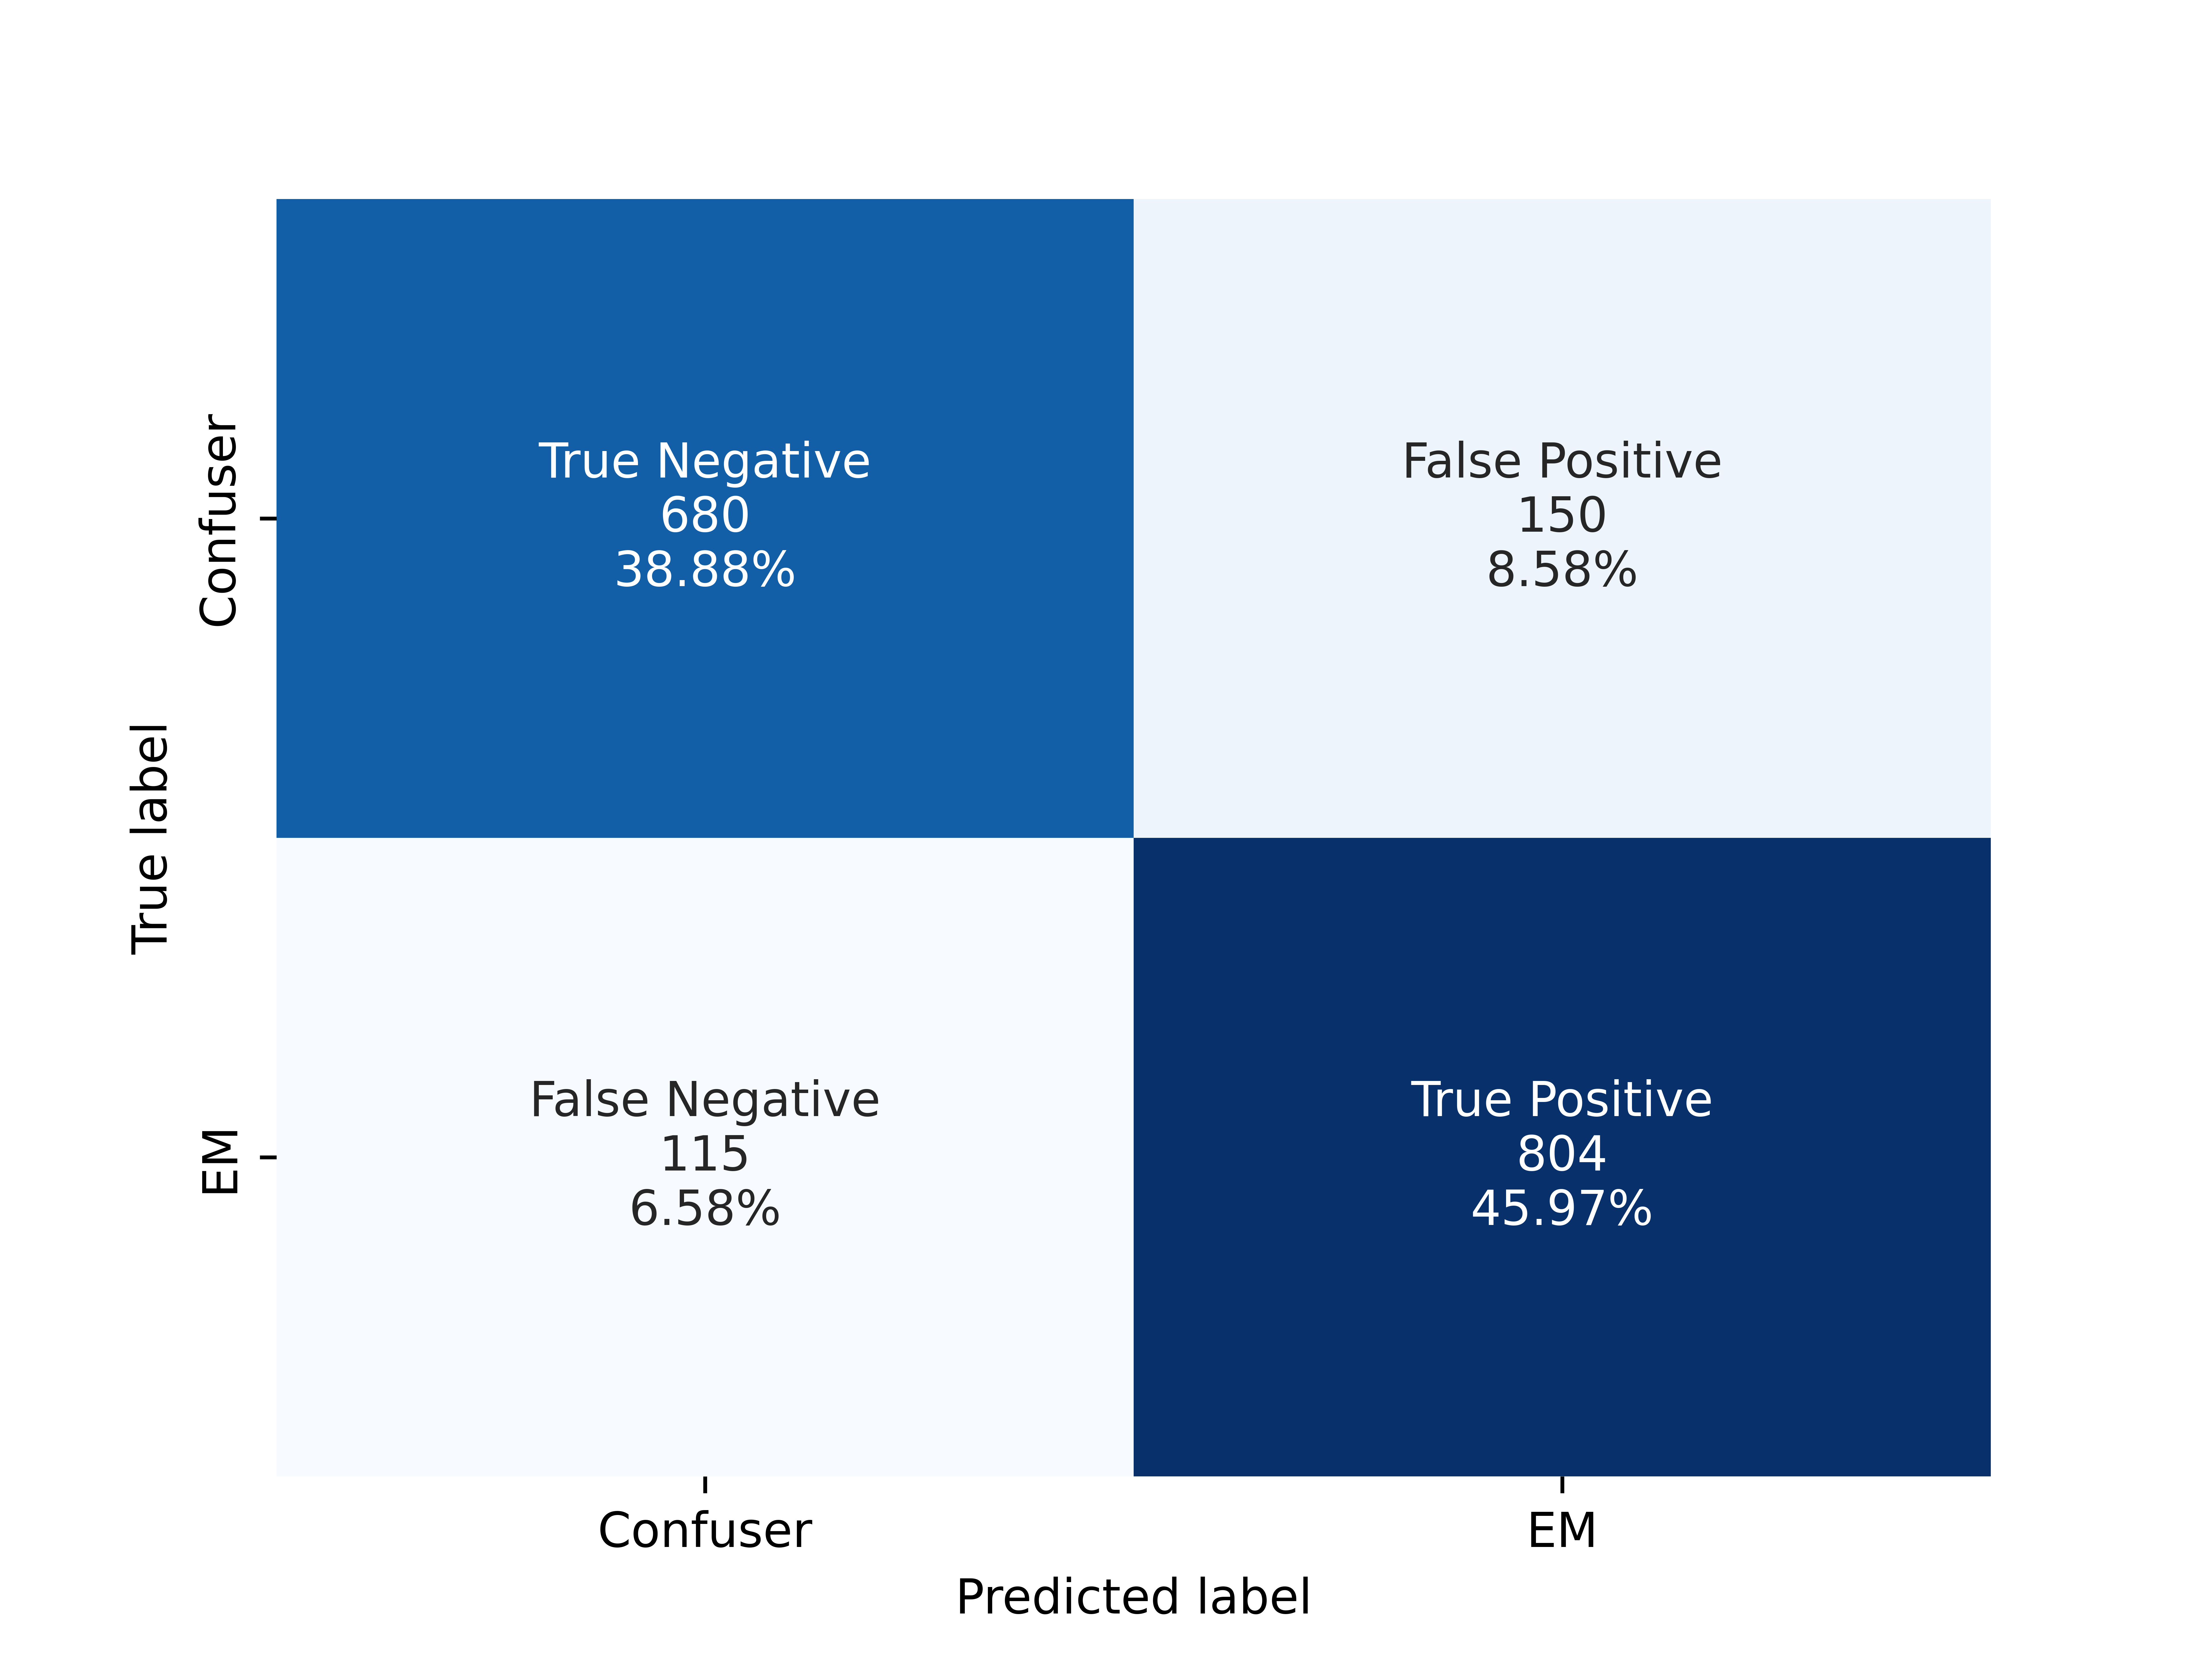
\includegraphics[width=\textwidth,keepaspectratio]{images/ongoing/ResNet50HAMIMGCOPYWEIGHTEC141DSV2logit_Combined_CM.png}
		\caption{Confusion matrix.}
	\end{subfigure}
	\caption{Five-fold cross-validation ROC curve and confusion matrix of ResNet50-141 model.}
\end{figure}
\resumetocwriting